
\section{Snakes and ladders : le jeu}

\textit{Extrait du travail de T. Kovaltchouk - UPSTI}

%\noindent \textbf{Notes}~: les importations des modules suivantes sont à réaliser~: \\
%\texttt{
%import random as r \\
%import math as m \\ 
%import numpy as np
%}

\subsection{Présentation du jeu}

Le jeu \emph{serpents et échelles} est un jeu de société où on espère monter les échelles en évitant de trébucher sur les serpents. Il provient d'Inde et est utilisé pour illustrer l'influence des vices et des vertus sur une vie.

\begin{figure}[h]
	\begin{center}
		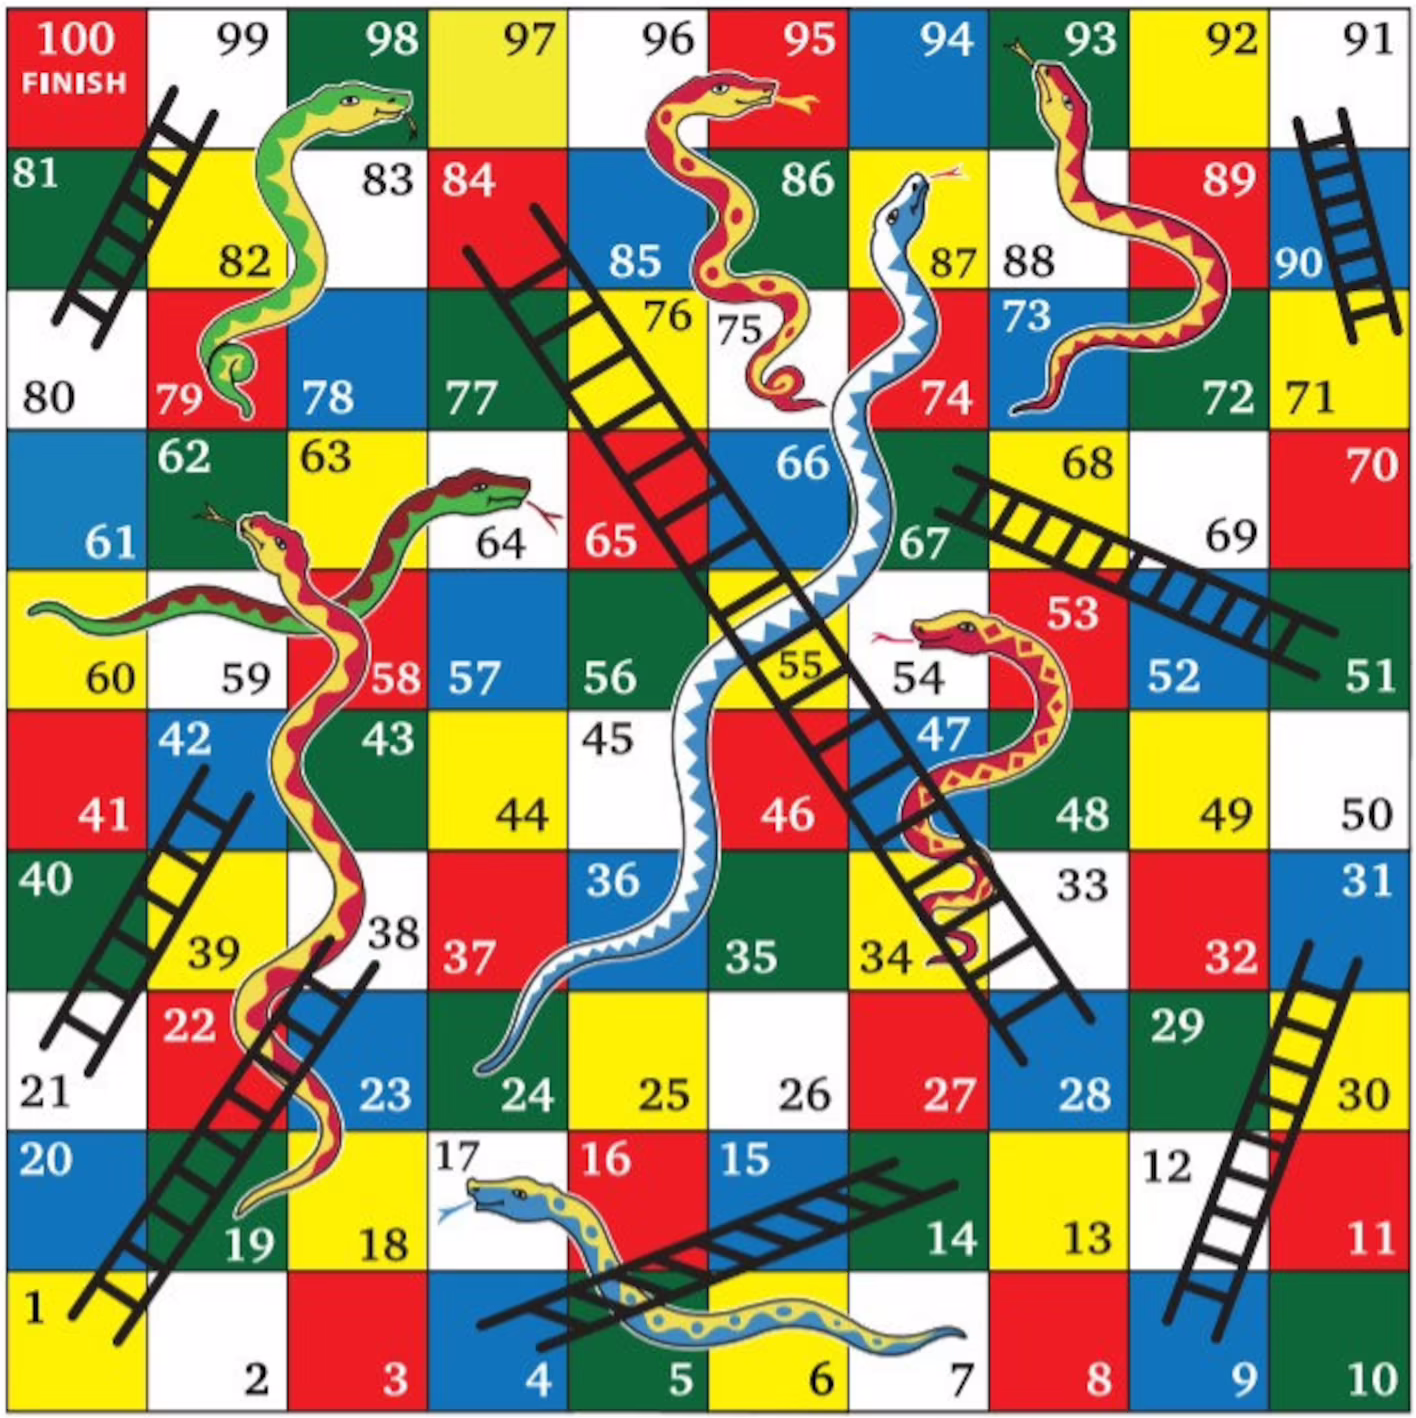
\includegraphics[width=0.6\linewidth]{snakesAndLadders}
	\end{center}
	\caption{Exemple d'un plateau de serpents et échelles}
	\label{fig:1}
\end{figure}

\paragraph*{Le plateau}

\begin{itemize}
	\item Le plateau comporte 100 cases numérotées de 1 à 100 en boustrophédon\footnote{à la manière du bœuf traçant des sillons, avec alternance gauche-droite et droite-gauche}~: le 1 est en bas à gauche et le 100 est en haut à gauche~;
	\item des serpents et échelles sont présents sur le plateau~: les serpents font descendre un joueur de sa tête à sa queue, les échelles font monter un joueur du bas de l'échelle vers le haut.
\end{itemize}

\paragraph*{Déroulement}

\begin{itemize}
	\item Chaque joueur a un pion sur le plateau. Plusieurs pions peuvent être sur une même case. Les joueurs lancent un dé à tour de rôle et ils avancent du nombre de cases marqués sur le dé. S'ils atterrissent sur un bas d'échelle ou une tête de serpent, ils vont directement à l'autre bout~;
	\item les joueurs commencent sur une case 0 hors du plateau~: la première case où mettre leur pion correspond donc au premier lancer de dé~;
	\item le premier joueur à arriver sur la case 100 a gagné~; 
	\item il existe 3 variantes quand la somme de la case actuelle et du dé dépasse 100~:
	\begin{itemize}
		\item le rebond~: on recule d'autant de cases qu'on dépasse~;
		\item l'immobilisme~: on n'avance pas du tout si on dépasse~: 
		\item la fin rapide~: on va à la case 100 quoi qu'il arrive. 
	\end{itemize}
\end{itemize}

On utilisera les notations suivantes pour les complexités~: $\indice{N}{cases}$, le nombre de cases du plateau (100), et $\indice{N}{SeE}$ la somme du nombre de serpents et du nombre d'échelle (16 dans notre exemple).

\subsection{Simulation du jeu}

\question{\'Ecrire une fonction \texttt{lancerDe() -> int} qui renvoie un nombre entier compris entre 1 et 6 en utilisant une fonction du module \texttt{random}. Vous pourrez vous aider des documentations en annexe.}


Les serpents et les échelles sont représentés par un dictionnaire \texttt{dSeE} tel que, pour une case de départ numérotée \texttt{i}, \texttt{dSeE[i]} donne le numéro de la case d'arrivée.

Avec l'exemple de la figure 1, on a~: 
\begin{lstlisting}
dSeE = {  1: 38,  4: 14,  9: 31, 17:  7, 21: 42, 28: 84, 51: 67, 54: 34, 
         62: 19, 64: 60, 71: 91, 80: 99, 87: 24, 93: 73, 95: 75, 98: 79}
\end{lstlisting}

\question{\'Ecrire la fonction \texttt{caseFuture(case: int) -> int} qui prend en argument le numéro de la case et qui renvoie le numéro de la case où va se trouver le joueur en atterrissant sur la case numérotée \texttt{case}. Par exemple, \texttt{caseFuture(5)} renvoie 5 (c'est un numéro de case stable), \texttt{caseFuture(1)} renvoie 38 (c'est un numéro de case avec échelle) et \texttt{caseFuture(17)} renvoie 7 (c'est un numéro de case avec une tête de serpent).}

%\UPSTIcorrection{
%	\lstinputlisting[firstline=22, lastline=26]{snakesAndLadder/simulationPartie.py}
%}

\question{Quelle est la complexité de cette fonction ?}

%\UPSTIcorrection{
%	Complexité en $O(1)$~: en effet, sur un dictionnaire, la recherche d'un clé dans un dictionnaire (\texttt{case in dSeE.keys()}) est en $O(1)$. 
%}

\question{\'Ecrire une fonction \texttt{avanceCase(case: int, de: int, choix: str) -> int} qui renvoie la case d'arrivée lorsqu'on part de la case \texttt{case} et qu'on a comme résultat au lancer du dé la valeur \texttt{de}. La variable \texttt{choix} est une chaine de caractère correspondant à la stratégie de fin différente~: \texttt{"r"} pour le rebond, \texttt{"i"} pour l'immobilisme et \texttt{"q"} pour une fin rapide. \label{Q:casesAccessibles}.}

%\UPSTIcorrection{
%	\lstinputlisting[firstline=28, lastline=38]{snakesAndLadder/simulationPartie.py}
%}


\question{Écrire une fonction \texttt{partie(choix: str) -> [int]} qui lance une partie à un joueur et renvoie la liste successive des cases visitées sur le plateau. Elle commencera donc forcément par \texttt{0} et finira forcément par \texttt{100}. Le choix du mode de fin est en argument, de façon similaire à la question précédente.} 

%\UPSTIcorrection{
%	\lstinputlisting[firstline=40, lastline=47]{snakesAndLadder/simulationPartie.py}
%}



%\FloatBarrier
\subsection{Plus court chemin}

On souhaite, dans cette partie, utiliser un algorithme glouton pour trouver la partie la plus courte. 

\question{\'Ecrire une fonction \texttt{casesAccessibles(case: int) -> [int]} qui renvoie la liste des 6 cases accessibles pour la case donnée en entrée. Vous utiliserez la fonction \texttt{avanceCase} de la question \ref{Q:casesAccessibles}. La liste renvoyée \texttt{cases} doit avoir le codage suivant~: \texttt{case[i]} doit correspondre à la case d'arrivée avec le résultat de dé \texttt{i+1} (donc la liste retournée doit toujours avoir une longueur de 6). On prendra l'option de fin rapide.}

%\UPSTIcorrection{
%	\lstinputlisting[firstline=22, lastline=26]{snakesAndLadder/partieGlouton.py}
%}


\question{Écrire une fonction \texttt{meilleurChoix(case: int) -> int} qui renvoie la meilleure case accessible depuis \texttt{case}. Il est interdit d'utiliser la fonction \texttt{max} dans cette question. }

%\UPSTIcorrection{
%	\lstinputlisting[firstline=28, lastline=34]{snakesAndLadder/partieGlouton.py}
%}


L'algorithme glouton consistera à choisir la valeur du dé permettant de maximiser son déplacement à chaque coup.

\question{Écrire une fonction \texttt{partieGloutonne() -> [int]} qui renvoie la liste des cases par lesquelles passe le pion dans l'algorithme glouton.}

%\UPSTIcorrection{
%	\lstinputlisting[firstline=36, lastline=42]{snakesAndLadder/partieGlouton.py}
%}

Cette dernière fonction nous renvoie \texttt{[0, 38, 44, 50, 67, 91, 97, 100]}. 

%\question{Construire un exemple de plateau, contenant par exemple 2 échelles et pas de serpent, pour lequel notre algorithme ne trouve pas le chemin le plus court en nombre de coups~: vous préciserez le résultat de l'algorithme glouton et un exemple d'une partie strictement plus rapide.}

%\UPSTIcorrection{
%	Soit une échelle qui va de 12 à 100 (donc arriver à 12 termine la partie) et une échelle qui va de 1 à 22~: l'algorithme glouton choisira d'aller sur la case 21 au départ, et finir avec une partie à 14 lancers, au lieu de faire 2 fois 6 et terminer la partie en seulement 2 lancers. 
%}


%\newpage

\section*{Annexe}

\subsection*{Utilisation du module \texttt{random}}

On vous donne les docstrings correspondant à deux fonctions du module \texttt{random}~: 

\begin{lstlisting}
randint(a, b) method of random.Random instance
    Return random integer in range [a, b], including both end points.
	
choice(seq) method of random.Random instance
    Choose a random element from a non-empty sequence.
\end{lstlisting}

\subsection*{Complexité des opérations sur les listes et dictionnaires}

\paragraph*{Principales opérations sur les listes}

\texttt{n}, longueur de la liste \texttt{L}, \texttt{k}, un indice valide en négatif (\texttt{1} à \texttt{n}).

\begin{longtable}{|m{9cm}|m{2.1cm}|} \hline
	\bf \centering Opération & \bf \centering Moyen \tabularnewline
	\hline
	\endhead
	Longueur (\texttt{len(L)}) &  $O(1)$ \tabularnewline
	\hline
	Accès en lecture d'un élément &  $O(1)$ \tabularnewline
	\hline
	Accès en écriture d'un élément &  $O(1)$ \tabularnewline
	\hline
	Copie (\texttt{L.copy()} ou \texttt{L[:]}) & $O(n)$ \tabularnewline
	\hline
	Ajout (\texttt{L.append(elt)} ou \texttt{L+=[elt]}) & $O(1)$ \tabularnewline
	\hline
	Extension (\texttt{L1.extend(L2)} ou \texttt{L1+=L2}) & $O(n_2)$ \tabularnewline
	\hline
	Concaténation (\texttt{L1 + L2}) &  $O(n_1 + n_2)$ \tabularnewline
	\hline
	Test de présence (\texttt{elt in L}) & $O(n)$ \tabularnewline
	\hline
	Désempiler dernier (\texttt{L.pop()}) &  $O(1)$ \tabularnewline
	\hline
	Désempiler autre (\texttt{L.pop(-k)}) &  $O(k)$ \tabularnewline
	\hline
	Maximum ou minimum (\texttt{max(L)} et \texttt{min(L)}) &  $O(n)$ \tabularnewline
	\hline
	Tri (\texttt{L.sort()} ou \texttt{sorted(L)}) &  $O(n \log(n))$ \tabularnewline
	\hline
\end{longtable}

\paragraph*{Principales opérations sur les dictionnaires}

\texttt{n}, longueur du dictionnaire \texttt{d}, \texttt{k}, une clé du dictionnaire.

\begin{longtable}{|m{9cm}|m{2.1cm}|} \hline
	\bf \centering Opération & \bf \centering Moyen \tabularnewline
	\hline
	\endhead
	Longueur (\texttt{len(d)}) &  $O(1)$ \tabularnewline
	\hline
	Accès en lecture d'un élément (\texttt{x = d[k]})  &  $O(1)$ \tabularnewline
	\hline
	Accès en écriture d'un élément (\texttt{d[k] = x}) &  $O(1)$ \tabularnewline
	\hline
	Copie (\texttt{d.copy()}) & $O(n)$ \tabularnewline
	\hline
	Ajout (\texttt{d[k] = x} la première fois) & $O(1)$ \tabularnewline
	\hline
	Test de présence (\texttt{k in d}) & $O(1)$ \tabularnewline
	\hline
	Retrait d'un élément (\texttt{del d[k]} ou \texttt{d.pop(k)}) & $O(1)$ \tabularnewline
	\hline
\end{longtable}

 


